\section{Objektdetektion}

Das folgende Kapitel befasst sich mit den ersten beiden Schritten in der automatisierten Analyse der Grabungsfotos: der Erkennung der Schiefertafeln und ihrer Extraktion aus dem Gesamtbild.\\
Zunächst werden verschiedene Möglichkeiten der Erkennung präsentiert und diskutiert. Der Schwerpunkt liegt hier auf dem schlussendlich umgesetzten Verfahren.
Abschließend wird das mit der Tafeldetektion verbundene Ausschneiden der gefundenen Tafeln aus dem Gesamtbild vorgestellt.

\subsection{Detektionsverfahren}

Aus den Anforderungen der Aufgabenstellung lässt sich als erster Arbeitsschritt die Detektion der Tafeln ableiten. Die wichtigste Prämisse ist dabei, dass Falsch-Negative, also nicht erkannte Tafeln, vermieden werden. Grund dafür ist, dass diese für die weitere Bearbeitung komplett verloren sind. Falsch-Positive sollten ebenfalls weitestgehend ausgeschlossen werden. Diese können jedoch in späteren Bearbeitungsschritten, vor allem der Texterkennung, erkannt und aussortiert werden. Daher ist dieses Kriterium von niedrigerer Priorität.
Dieses Kapitel wird sich daher verschiedenen Verfahren widmen, mit denen rechteckige, beschriftete Objekte erkannt werden können. Diese Verfahren werden vorgestellt und ihre Ergebnisse in einer ersten, explorativen Umsetzung präsentiert. Anschließend wird begründet, warum diese Verfahren im Rahmen des Projektes nicht nicht zum Einsatz kommen. Final wird dann das Kontur-basierte Erkennungsverfahren erläutert, mit dem die besten Ergebnisse erzielt wurden.

%das Kapitel wird aus einer Kurzvorstellung der einzelnen Ansätze bestehen, die in Frage kamen und ausprobiert wurden
%In der Tiefe wird sich anschließend mit dem letztlich umgesetzten Verfahren, basierend auf \verb|cv2.contours|, auseinandergesetzt.

\subsubsection{Feature Detection}

was ist feature detection?
wie funktioniert sie?
was war die Idee hinter dem Ansatz?
Wie sehen die Ergebnisse aus?

\subsubsection{CNN}

hier werden CNNs vorgestellt
was sind CNNs?
Was können sie, wie funktionieren sie?
Warum habe ich sie ausprobiert, was war die Idee dahinter?
Warum habe ich nicht selbst trainiert?
Wie sehen die Ergebnisse aus?

\subsubsection{Contours}

\verb|Cv2.Contours| basiert auf einem Algorithmus, der Punkte gleicher Farbe und Intensität umrandet \cite{suzuki}. Das Resultat ist eine Liste von Punkten, die ein geschlossenes Polygon ergeben. Die gefundenen Konturen können mit einer Hierarchie versehen werden, bei der Konturen, die sich innerhalb anderer Konturen befinden, als deren \glqq Kinder\grqq gelten. Das Verfahren ist darauf ausgelegt, auf binäre Bilder angewendet zu werden. Die Implementierung in OpenCV unterscheidet in Nullwerte und Nicht-Nullwerte \cite{opencvcontours}. Nicht-binäre Bilder werden also automatisch binarisiert. Für die Erzielung optimaler Ergebnisse kommt dem Binarisierungsverfahren allerdings eine große Bedeutung zu.
Auf Basis dieses Algorithmus lässt sich Detektionsverfahren aufbauen, das Objekte, die sich vom Hintergrund der Bilder abheben, zu erkennen. Die Herausforderung besteht, nach diesem Ansatz, in zwei Punkten: Erstens muss die Binarisierung so erfolgen, dass eine möglichst saubere Trennung von Vordergrund (Objekten) und Hintergrund (vor allem Erde) der Bilder stattfindet und zweitens müssen aus den gefundenen Vordergrundobjekten diejenigen ausgewählt werden, die als Tafeln in Frage kommen. Wie bereits erwähnt hat dabei die Vermeidung Falsch-Negativer eine höhere Priorität als die von Falsch-Positiven. Bei der Binarisierung haben sich zwei Wege als praktikabel herausgestellt, die im Folgenden beide präsentiert werden sollen. Im Flowchart sind die Abläufe der Rechtecksdetektion schematisch dargestellt (Vgl. Abb.\ref{fig:flowrectdetect}).
\begin{figure}[h!]
\centering
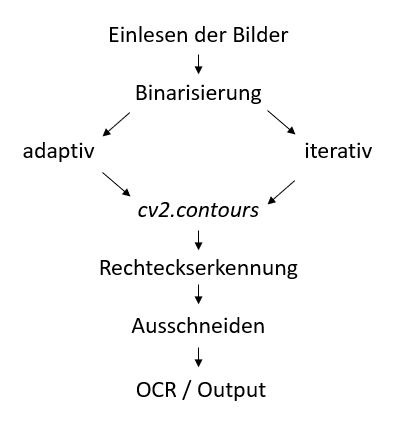
\includegraphics[width =0.5\textwidth]{flowchart_cont.PNG}
\caption{Flowchart Rechteckserkennung.}
\label{fig:flowrectdetect}
\end{figure}

\subsubsection*{Adaptive Binarisierung}

Das einfachste Verfahren der Binarisierung eines Bildes besteht darin, einen Threshold, also einen Grenzwert festzulegen. Dieser muss auf der Spanne der Farbwerte, also zwischen 0 und 255 liegen.  Farbwerte unterhalb dieses Thresholds werden zu Nullen, Farbwerte darüber zu Einsen. Das Ergebnis ist ein reines Schwarz-Weiß-Bild. Bei komplexen Szenerien, wie den Grabungsfotos, ist dieses Verfahren jedoch zu einfach. So kann ein Foto beispielsweise stark unterschiedliche Beleuchtung, wie direktes Sonnenlicht und Schatten, enthalten. Eine Differenzierung innerhalb dieser Zonen ist so nicht möglich (Vgl. Abb. \ref{fig:threshold}).\\
\begin{figure}[h!]
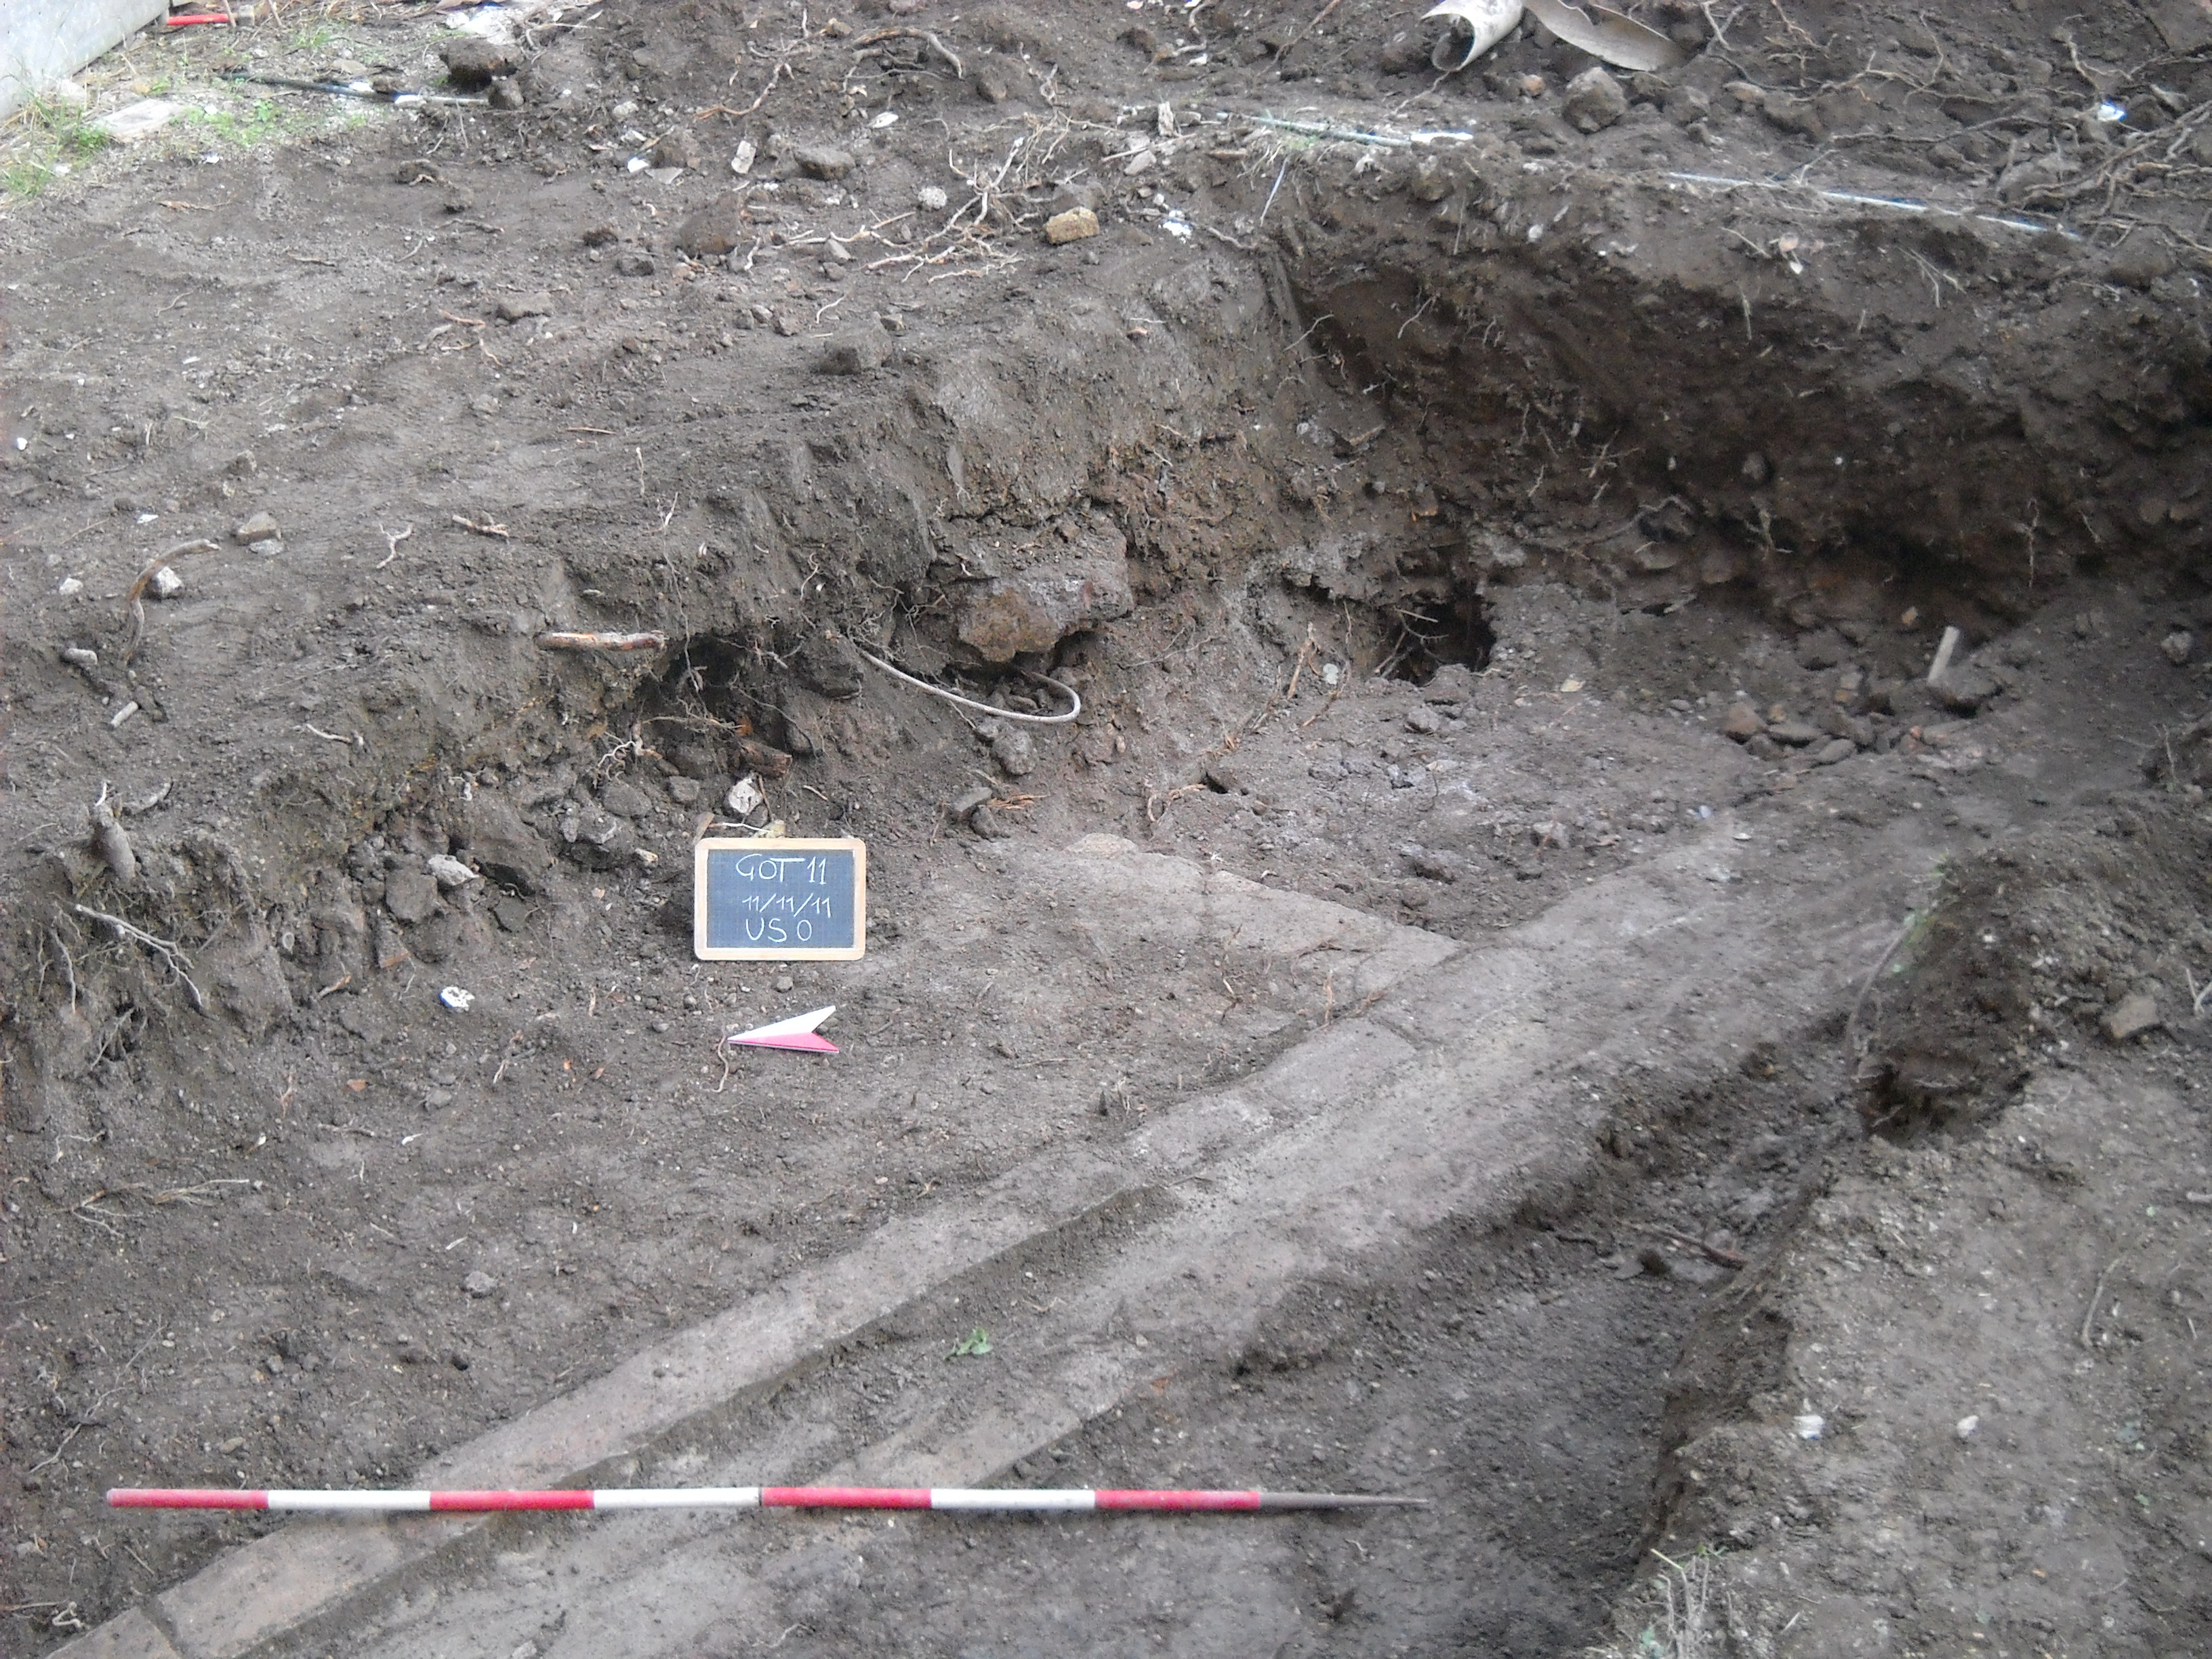
\includegraphics[width =0.5\textwidth]{catacom_1020.JPG}
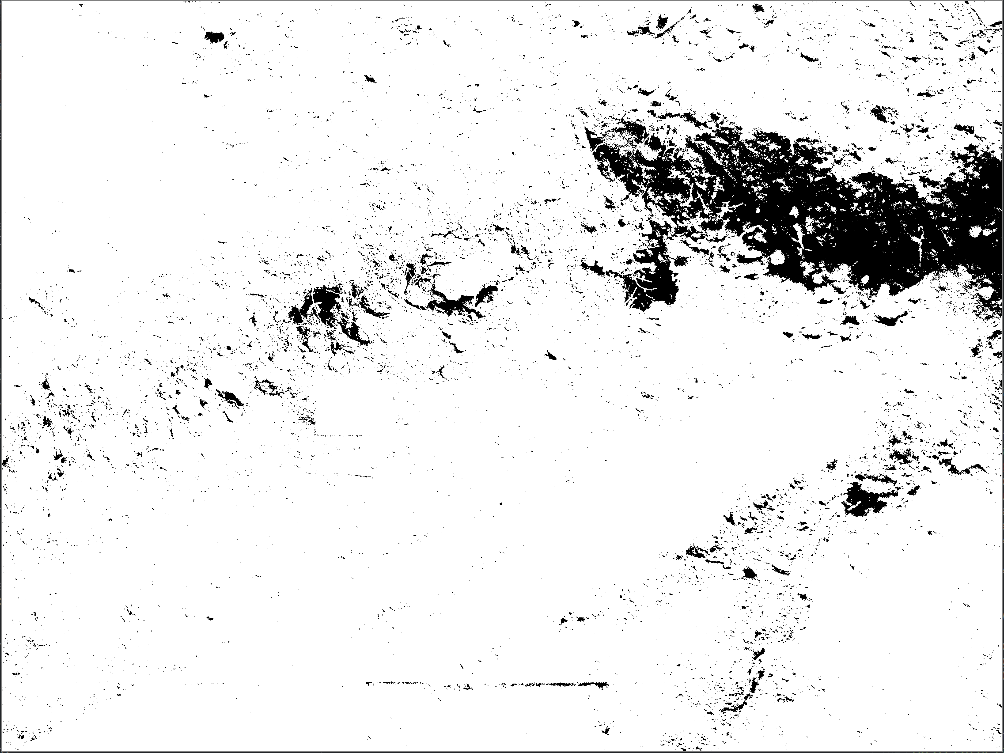
\includegraphics[width =0.5\textwidth]{thresh60.png}
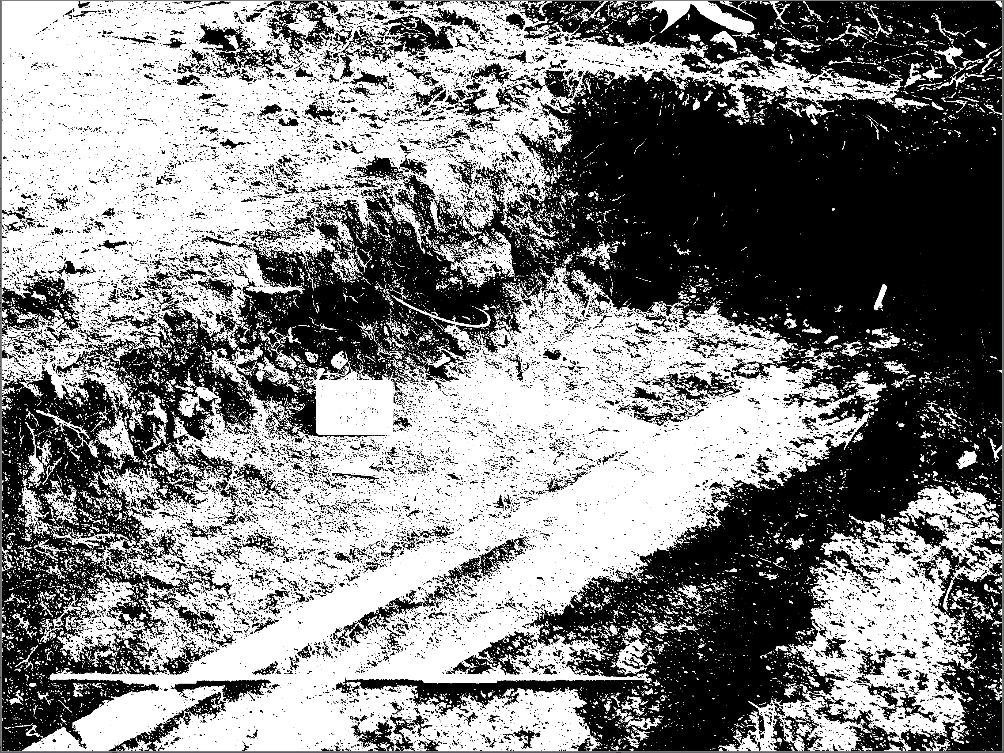
\includegraphics[width =0.5\textwidth]{thresh125.png}
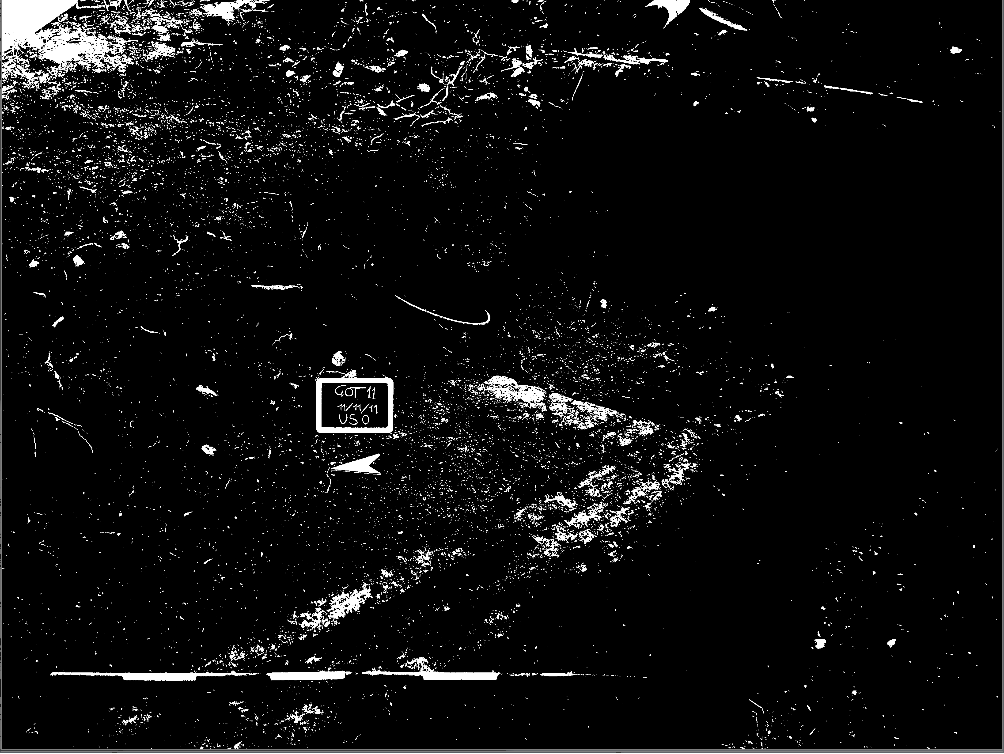
\includegraphics[width =0.5\textwidth]{thresh185.png}
\caption{Grabungsfoto im Original (o.l.), mit niedrigem (60, o.r.), mittlerem (125, u.l.) und hohem (185, u.r.) Threshold.}
\label{fig:threshold}
\end{figure}
Eine Lösung für dieses Problem ist die Anwendung eines adaptiven Thresholds \cite{opencvadaptivethresholdopencvadaptivethreshold}): Statt global, über das gesamte Bild, einen Grenzwert festzulegen, können lokale Grenzwerte errechnet werden. Die Größe des lokalen Ausschnittes sowie das exakte Verfahren können dabei frei gewählt werden. In diesem Fall wird für die Binarisierung ein Gauss-Verfahren auf einen Kernel von 11 x 11 Pixeln angewendet. Die Beleuchtung oder Farbunterschiede innerhalb des Bildes können so ausgeglichen werden (Vgl. Abb. \ref{fig:adaptivethreshold}).
\begin{figure}[h!]
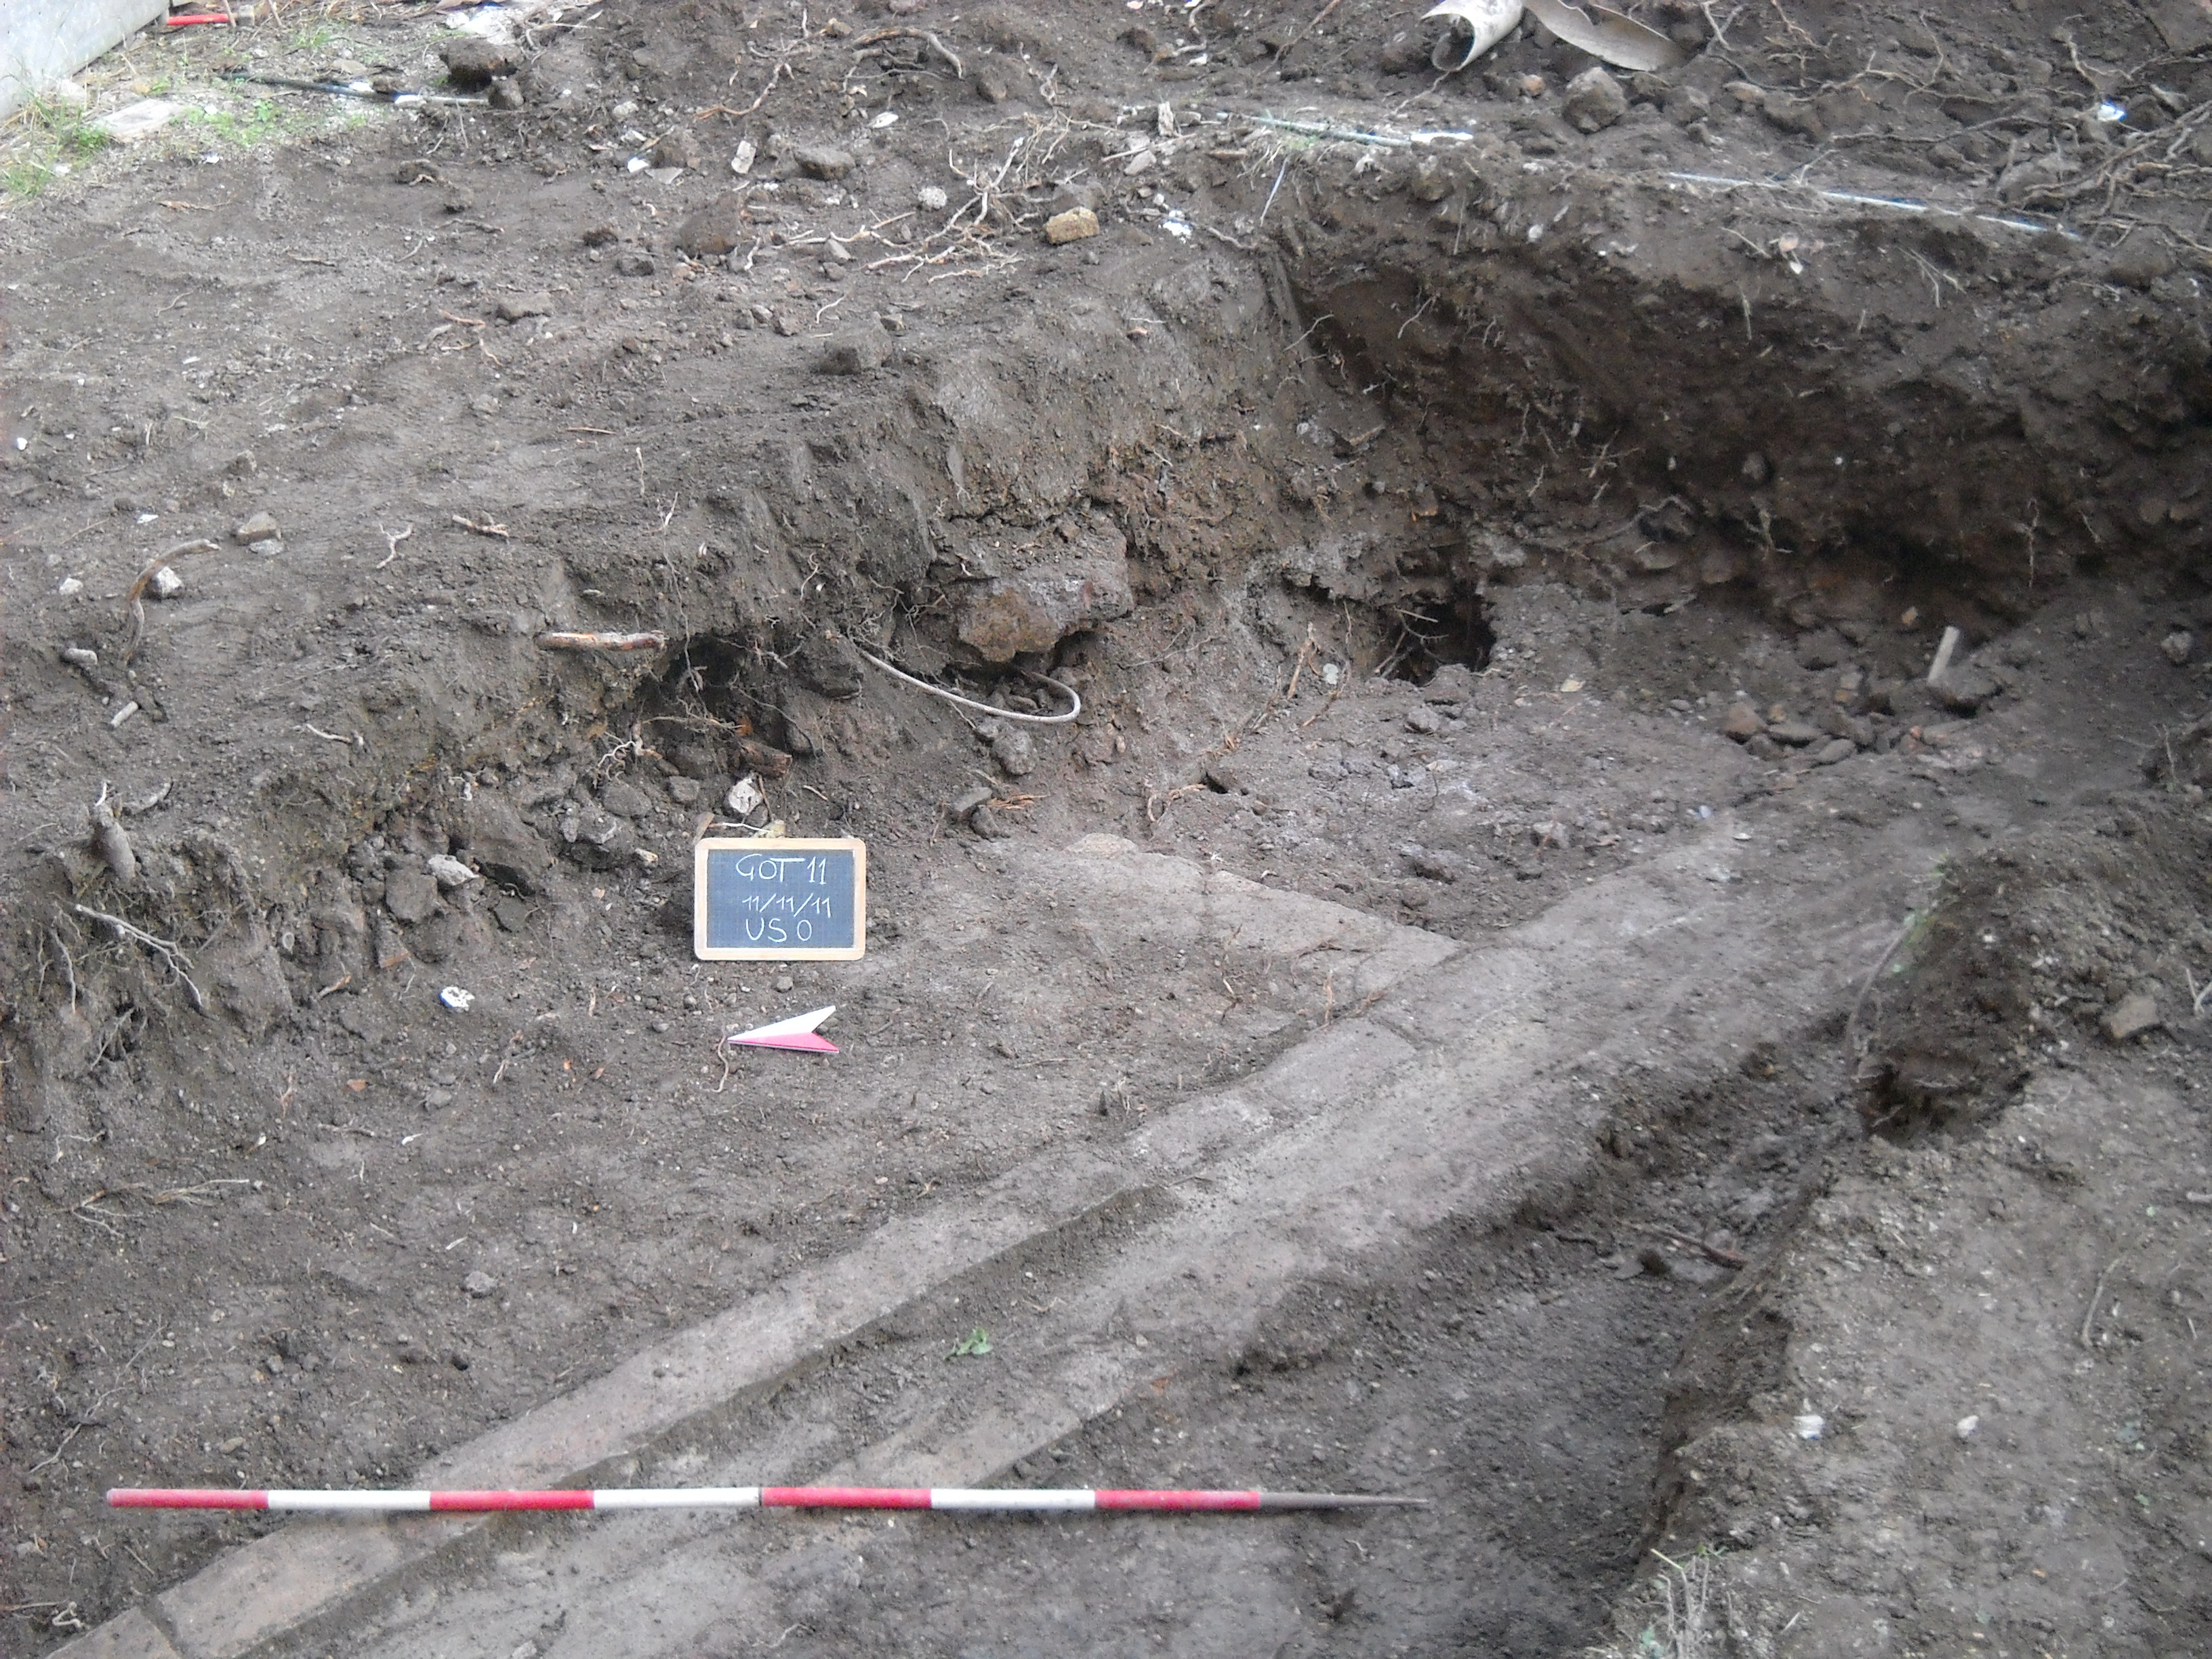
\includegraphics[width =0.5\textwidth]{catacom_1020.JPG}
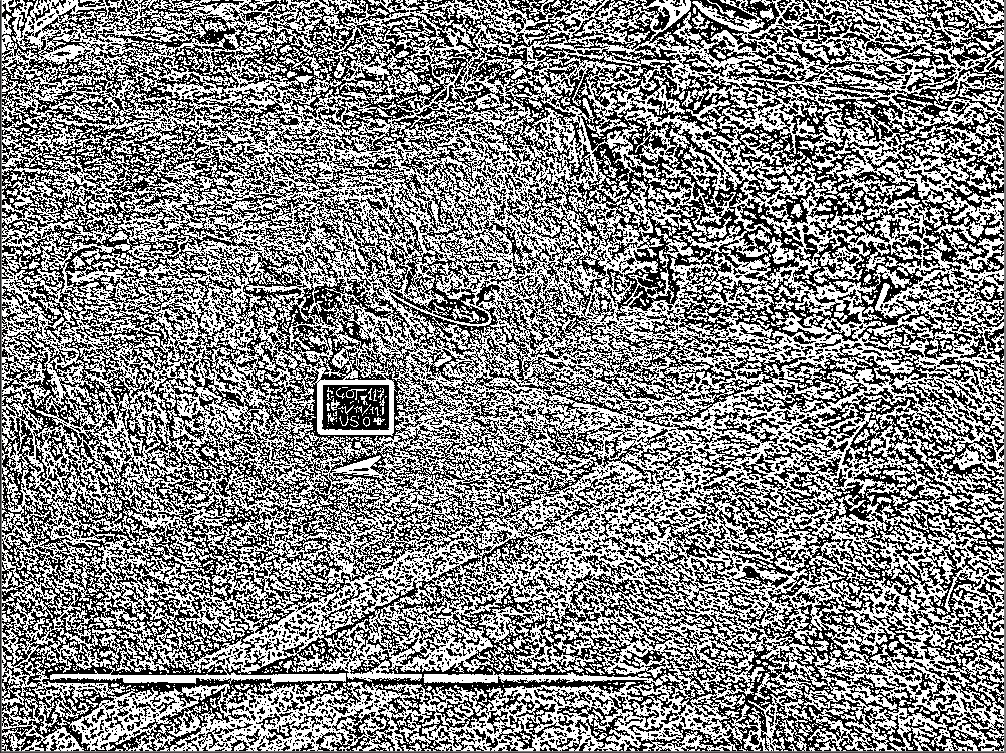
\includegraphics[width =0.5\textwidth]{adaptivethreshold.png}
\caption{Grabungsfoto im Original sowie mit adaptivem Threshold.}
\label{fig:adaptivethreshold}
\end{figure}
Vor der Binarisierung muss das Bild in ein Grauskala-Bild umgewandelt verkleinert\footnote{Genauer: Der längere Bildrand wird auf 1000 Pixel reduziert, der kürzere entsprechend angepasst. Die Grabungsfotos haben in der Regel eine Auflösung von 3264 x 2448 Pixeln. Es findet also eine Reduktion auf ca. $\frac{1}{10}$ der Fläche statt. Bilder kleiner als 1000 Pixel würden theoretisch auf 1000 Pixel vergrößert werden. Da für die hier beschriebenen Prozesse und vor allem für die Texterkennung später aber eine gewisse Bildqualität erforderlich ist, ist von diesem Fall nicht auszugehen.}. Das verbessert die Genauigkeit der Detektion und verringert die zu verarbeitende Datenmenge, wodurch der Prozess beschleunigt wird. Die Verkleinerung des Bildes ist allerdings ein Prozess, der später rückgängig gemacht werden muss, um Datenverlust bei der Texterkennung zu verhindern.

\subsubsection*{Iterative Binarisierung}

Die adaptive Binarisierung bringt einige Nachteile mit sich. So ist hier die Erkennung von Falsch-Positiven relativ hoch. Die Konturen werden auf einem verkleinerten Bild gesucht und müssen später auf Originalgröße skaliert werden, was ein verlustbehafteter Prozess ist. Daher gibt es einen zweiten Ansatz, hier als iterativer Ansatz bezeichnet. Die Grundidee besteht darin, das Bild mit einem globalen Threshold zu binarisieren. Die Problematik davon wurde bereits diskutiert: Bei großen Beleuchtungsunterschieden oder sehr hellen oder dunklen Objekten auf dem Bild werden ganze Bereiche durch den Threshold von der weiteren Bearbeitung ausgeschlossen. Der iterative Ansatz sieht daher vor, den Threshold von 20 auf 200 in Fünferschritten zu erhöhen. Dadurch entstehen pro Foto 37 binäre Bilder, auf die die Konturenerkennung angewendet werden kann. Auf jedem dieser Bilder können mehrere mögliche Tafeln erkannt werden\footnote{Die eigentliche Tafelerkennung wird erst im folgenden Abschnitt beschrieben. Da die dort gewonnenen Informationen nicht, wie beim adaptiven Ansatz, an das Hauptprogramm übergeben, sondern innerhalb der Funktion des iterativen Ansatzes weiter verarbeitet werden, ist hier ein Vorgriff nötig.}. Der nächste Schritt besteht also darin, aus diesen möglichen Tafeln die auszuwählen, die am wahrscheinlichsten tatsächlich eine ist. In diesem Kontext wird eine Grundannahme getroffen: Es wird davon ausgegangen, dass in dem Bereich, in dem auf den meisten der 37 Bilder eine Tafel vermutet wird, sich tatsächlich eine Tafel befindet. Alle anderen werden als Falsch-Positive betrachtet. Diese Annahme beruht auf zwei Faktoren: Erstens hat sich gezeigt, dass Objekte, die keine Tafeln sind, aber als solche erkannt werden können -- beispielsweise Fenster, Türen oder Plakate -- nur unter wenigen Thresholds als solche eingeordnet werden. Das liegt unter anderem darin begründet, dass die Tafeln einen hellen Holzrahmen und eine dunkle Innenfläche haben, was zu einem starkem Kontrast führt, der auf vielen Stufen des Thresholds erhalten bleibt\footnote{Die Tafeln verfügen damit über eine Eigenschaft, die auch beim Einsatz von AR-Markern genutzt wird: Starke hell-dunkel Kontraste beschleunigen und vereinfachen die Detektion \cite[p.~45]{armarker}}. Zweitens werden durch eben diesen Rahmen in mittleren Threshold-Bereichen die Tafeln oft zweimal erkannt: Einmal an der Außenkante und einmal an der Innenkante des Rahmens. Dadurch häuft sich die Detektion möglicher Tafeln in diesem Bereich.
Basierend auf dieser Annahme wird auf alle möglichen Tafeln immer paarweise die \verb|intersection over union| angewendet. Dieser Algorithmus basiert auf dem Jaccard-Koeffizienten zur Berechnung der Ähnlichkeit zweier Mengen \cite{intersectionoverunion}. Der Koeffizienten wird errechnet, indem die Schnittmenge durch die Vereinigungsmenge geteilt wird. Das Ergebnis liegt zwischen 0 und 1. Je mehr es sich der 1 annähert, desto ähnlicher sind die Mengen. Diese Berechnung lässt sich auch auf die Rechtecke, mit denen die möglichen Tafeln verortet werden, anwenden (Vgl. Abb. \ref{fig:jaccard}).

\begin{figure}[h!]
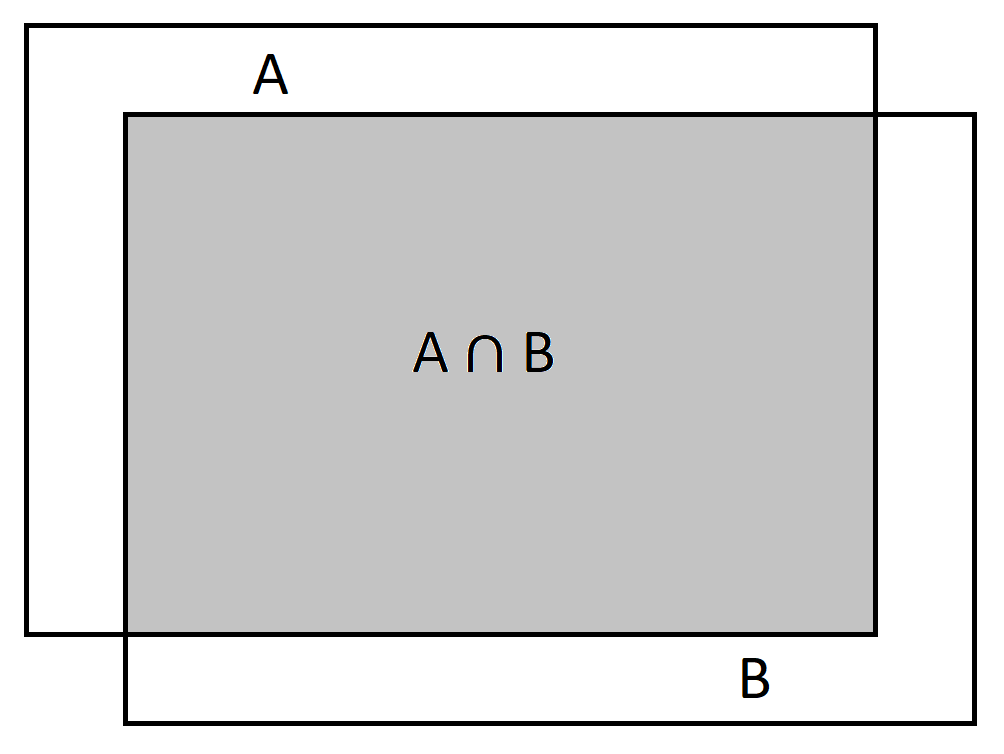
\includegraphics[width =0.5\textwidth]{schnittmenge.png}
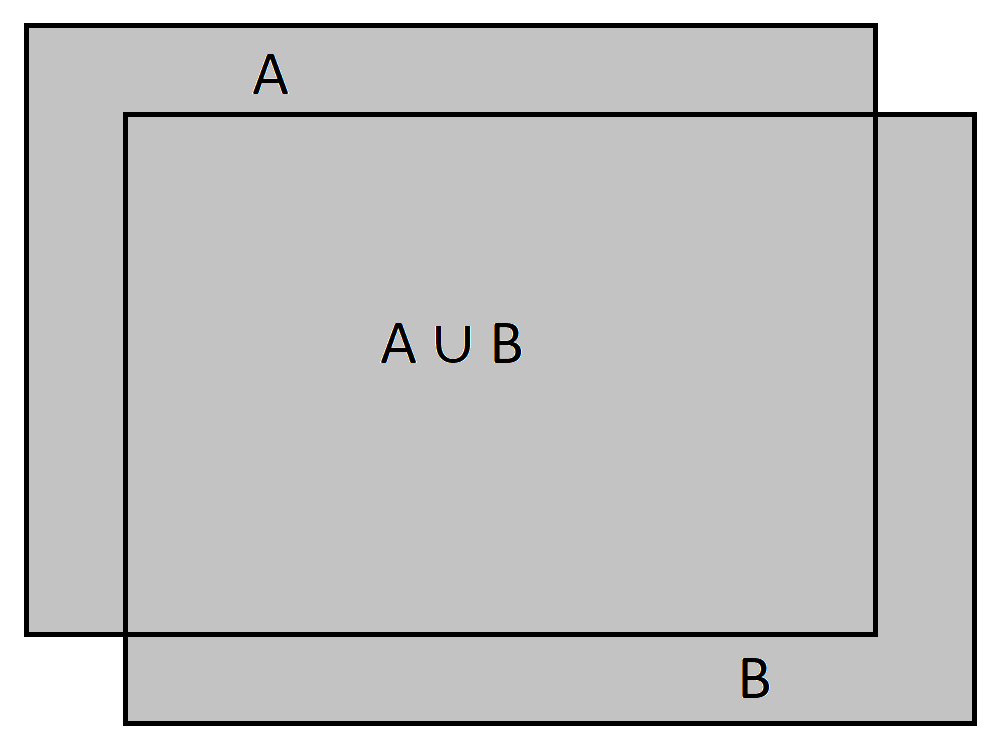
\includegraphics[width =0.5\textwidth]{vereinigungsmenge.png}
\caption{Schnittmenge und Vereinigungsmenge.}
\label{fig:jaccard}
\end{figure}

Im Rahmen dieses Projekts gelten zwei Rechtecke dann als hinreichend ähnlich, wenn der Jaccard-Koeffizient über 0.9 liegt. Jedes Mal, wenn ein Rechteck im Vergleich mit einem anderen diesen Wert erzielt, wird für das Rechteck ein Zähler erhöht. Das Rechteck, welches am Ende der Vergleiche den höchsten Wert in diesem Zähler erzielt, wird als tatsächliche Tafel angenommen. Eine Ausnahme ergibt sich, wenn dieser Wert unter 6 liegt. In diesem Falle, so hat sich ergeben, handelt es sich ausschließlich um Falsch-Positive. Je höher der Wert, desto sicherer ist die Identifikation der Tafel. Unter guten Bedingungen erreicht er Werte um die 20.

\subsubsection*{Rechteckserkennung}

Ist die Binarisierung der Bilder nach einer der beiden vorgestellten Methoden erfolgt, können mittels \verb|cv2.findContours| die Konturen der Objekte darauf gefunden werden (Vgl. Abb. \ref{fig:adaptivecont}). Die Hierarchie der Konturen wird dabei außer Acht gelassen, da sich daraus keine verlässlichen Informationen gewinnen lassen.
\begin{figure}[h!]
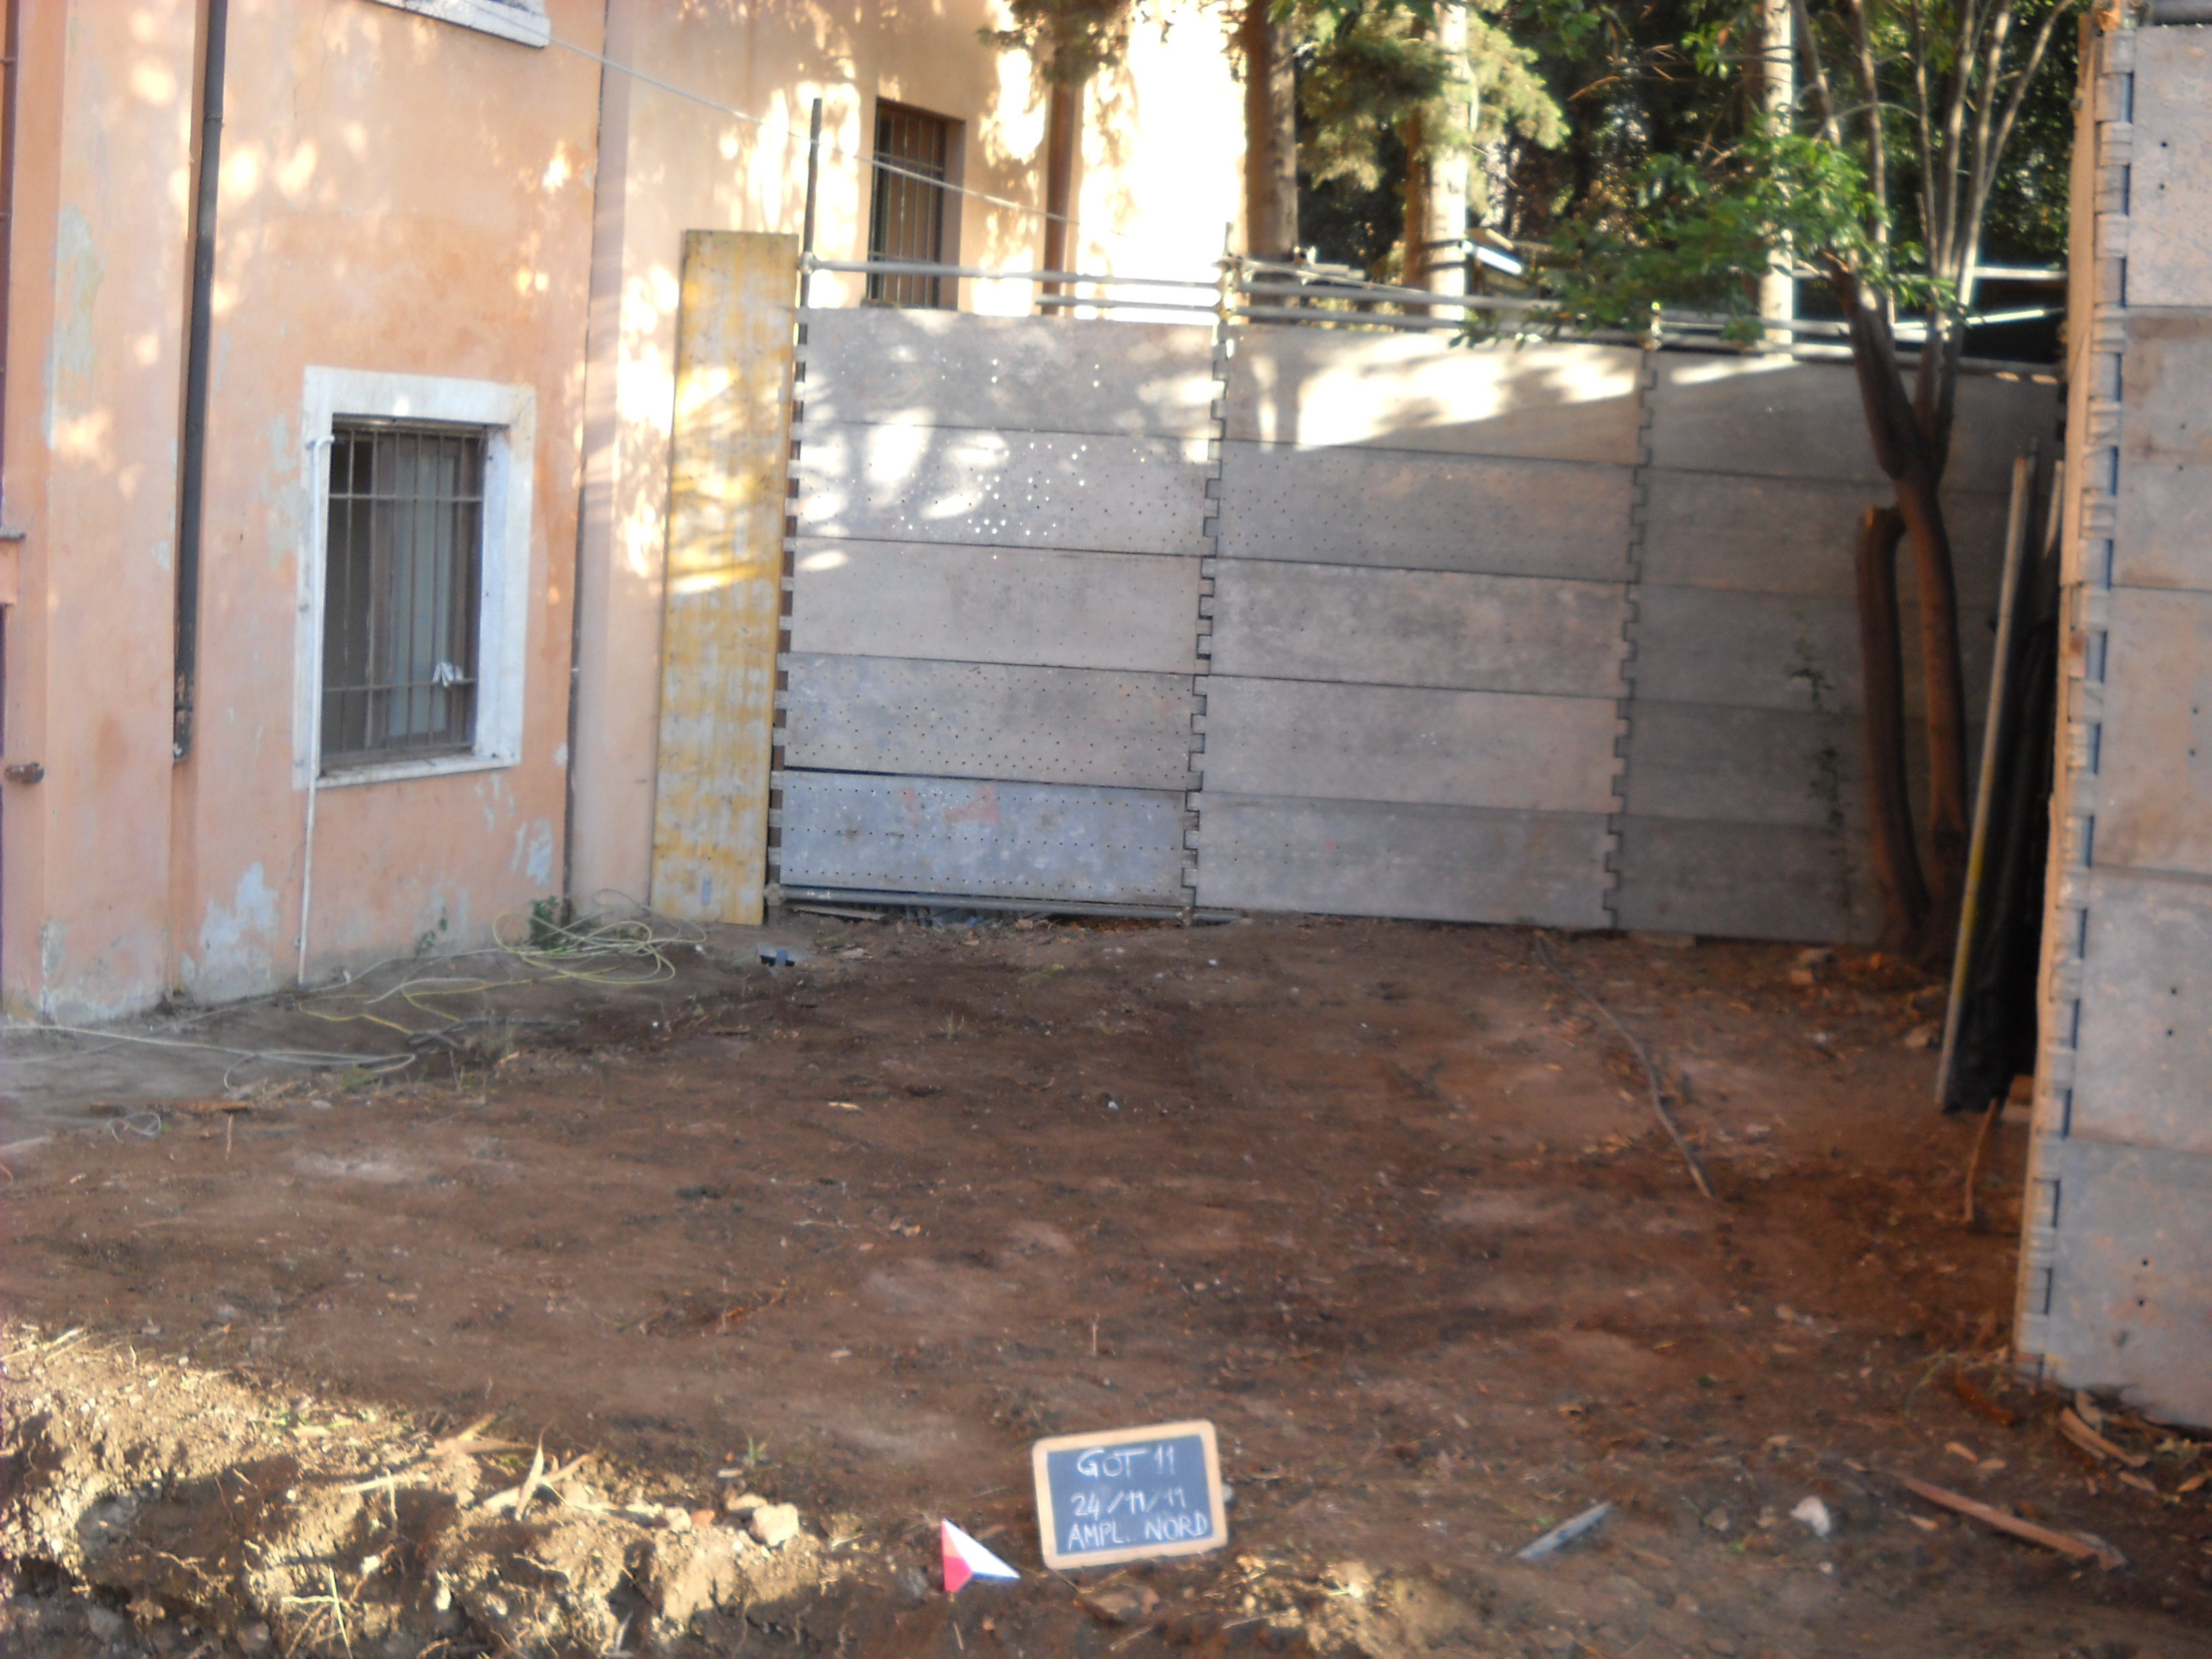
\includegraphics[width =0.5\textwidth]{catacom_1111.JPG}
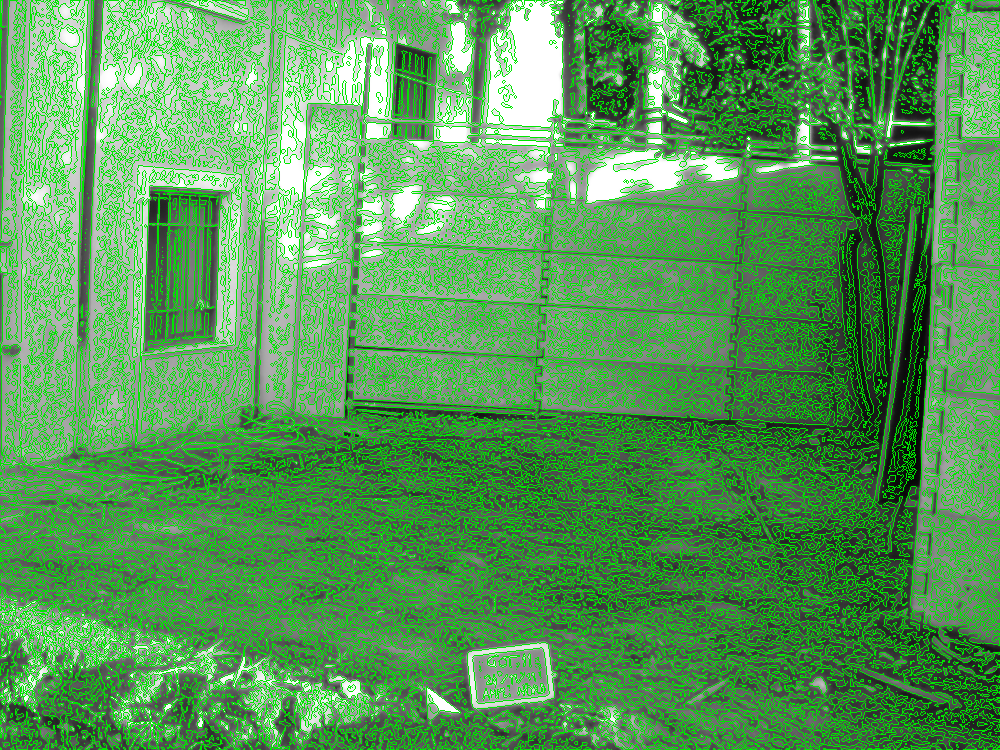
\includegraphics[width =0.5\textwidth]{catacom_1111_adaptive_cont.png}
\caption{Grabungsfoto im Original sowie nach der Anwendung der Konturerkennung.}
\label{fig:adaptivecont}
\end{figure}
%Zweispurigkeit der Ansätze: iterativ und adaptiv. Erklären warum.
%\verb|rect_detect| als Finale, in dem die beiden Ansätze wieder zusammengeführt werden
Als nächstes müssen unter diesen Konturen die ausgewählt werden, die als Tafel in Frage kommen. Dazu wird die Tatsache genutzt, dass es sich bei den Tafeln um Gegenstände handelt, die auf den Fotos als Rechtecke abgebildet werden. Durch ihre Lage zur Kamera können sie zu einem gewissen Grad davon abweichen, grundsätzlich bleibt diese Form aber annähernd erhalten. Andere Rechtecke kommen zwar vor, wie Plakate, Fenster, Türen, Ziegel und Fliesen, unterscheiden sich jedoch meist signifikant in der tatsächlichen Form oder können im Zweifelsfall bei der späteren Texterkennung ausgeschlossen werden. Dementsprechend geht es in der weiteren Tafelerkennung darum, Rechtecke zu finden und diese durch verschiedene weitere Kriterien so zu sortieren, dass alle Tafeln und möglichst nur Tafeln erkannt werden. Das wird in mehreren Schritten erreicht:
Zunächst wird die Fläche der Konturen berechnet. Genutzt wird hierfür die OpenCV-Funktion \verb|cv2.contourArea|. Ist diese Fläche zu klein, wird die Kontur aussortiert. Als Vergleichswert wird hier die Kantenlänge der längsten Kante des Bildes genommen, damit bei höherer Auflösung weiterhin korrekt sortiert werden kann(Vgl. Abb. ref{fig:adaptivecontsize}). Eine Größenbegrenzung ist sinnvoll, da die Tafeln in der Regeln eher prominent im Bild zu sehen sind. Sollte tatsächlich eine Tafel durch dieses Kriterium aussortiert werden, wäre der Text darauf nicht mehr lesbar und somit ohnehin nicht interessant für die weitere Verarbeitung.
\begin{figure}[h!]
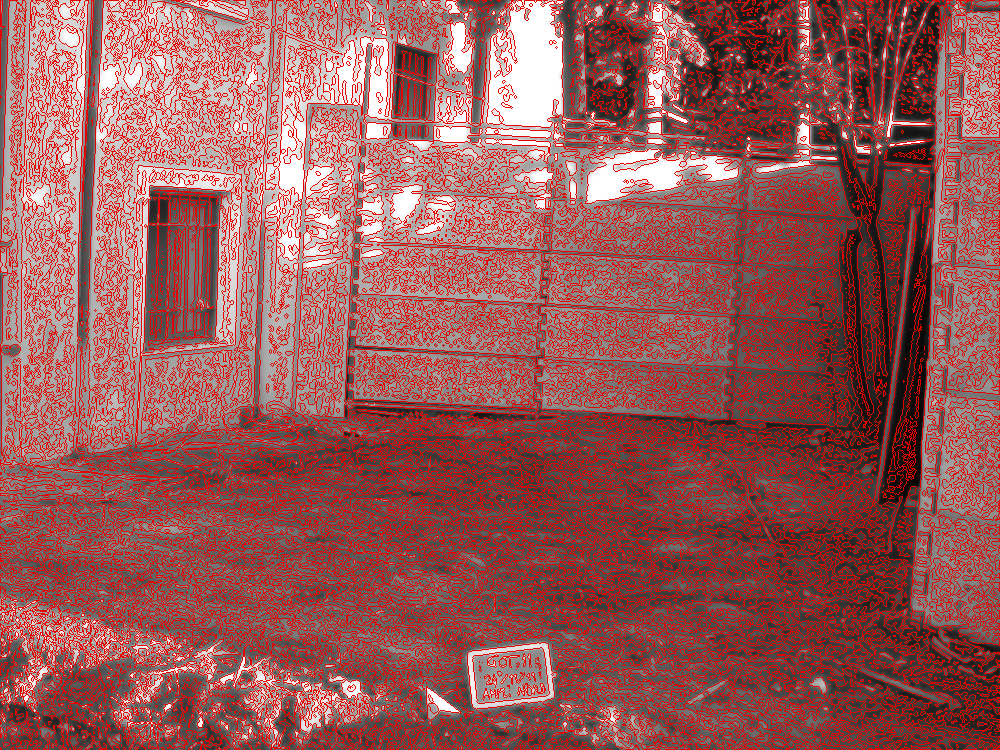
\includegraphics[width =0.5\textwidth]{catacom_1111_adaptive_contred.png}
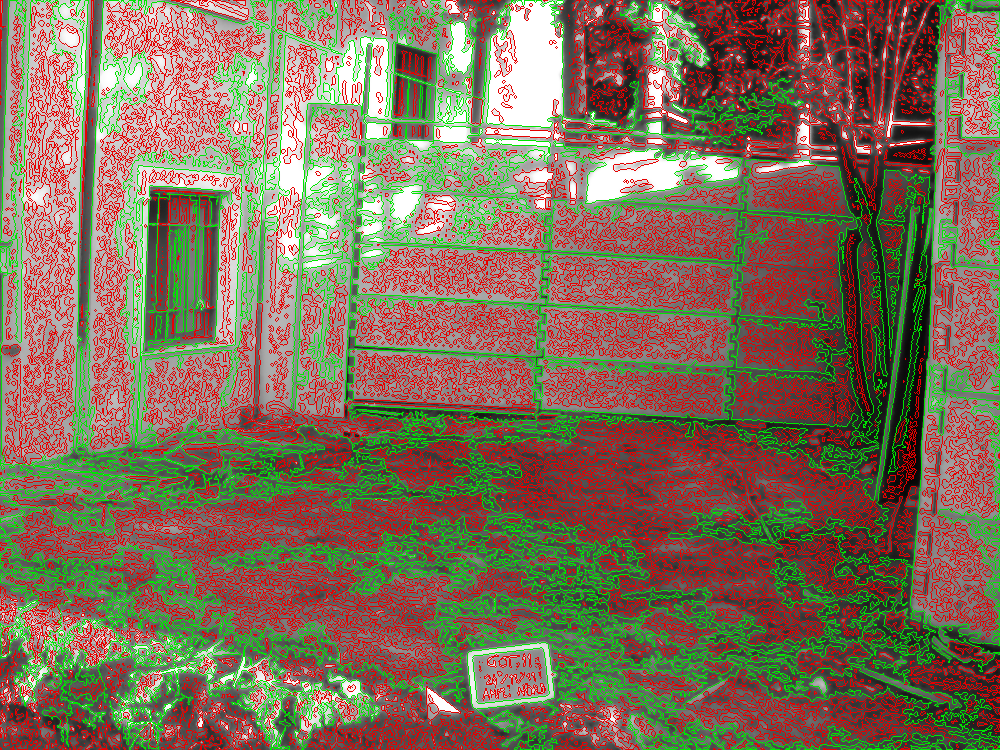
\includegraphics[width =0.5\textwidth]{catacom_1111_adaptive_bigcont.png}
\caption{Konturen vor und nach der Selektion nach Fläche.}
\label{fig:adaptivecontsize}
\end{figure}

Der nächste Schritt besteht darin, das kleinstmögliche Rechteck um die Kontur zum bilden. Auch hier kommt mit \verb|cv2.minAreaRect| eine Bibliotheksfunktion zum Einsatz (Vgl. Abb. \ref{fig:adaptiverectangles}).
\begin{figure}[h!]
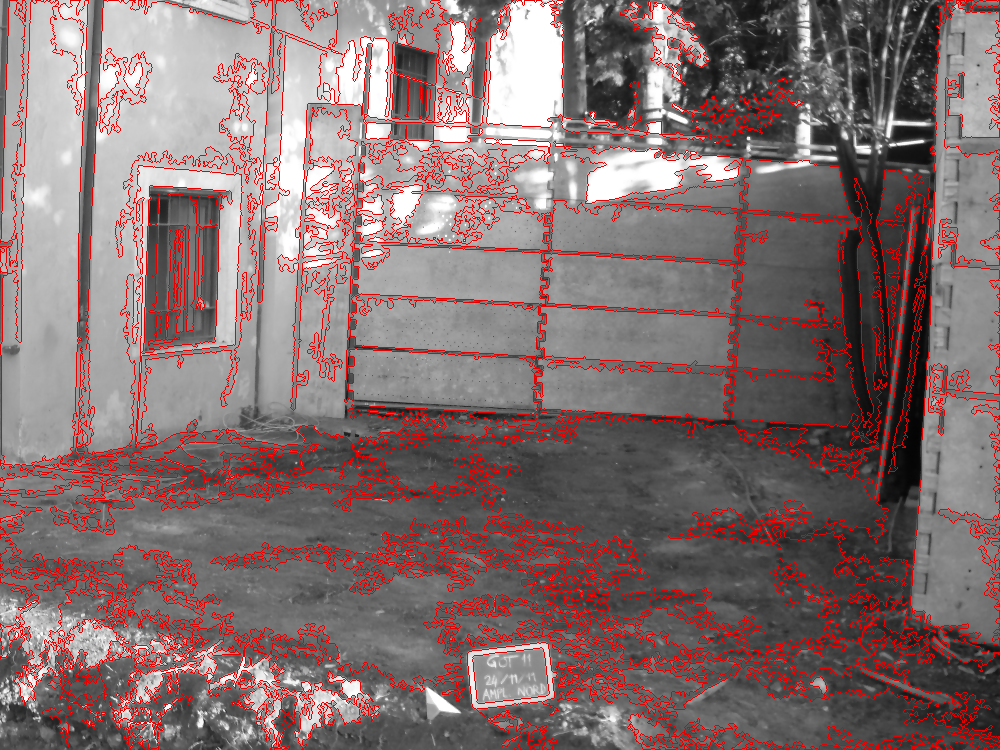
\includegraphics[width =0.5\textwidth]{catacom_1111_adaptive_bigcontred.png}
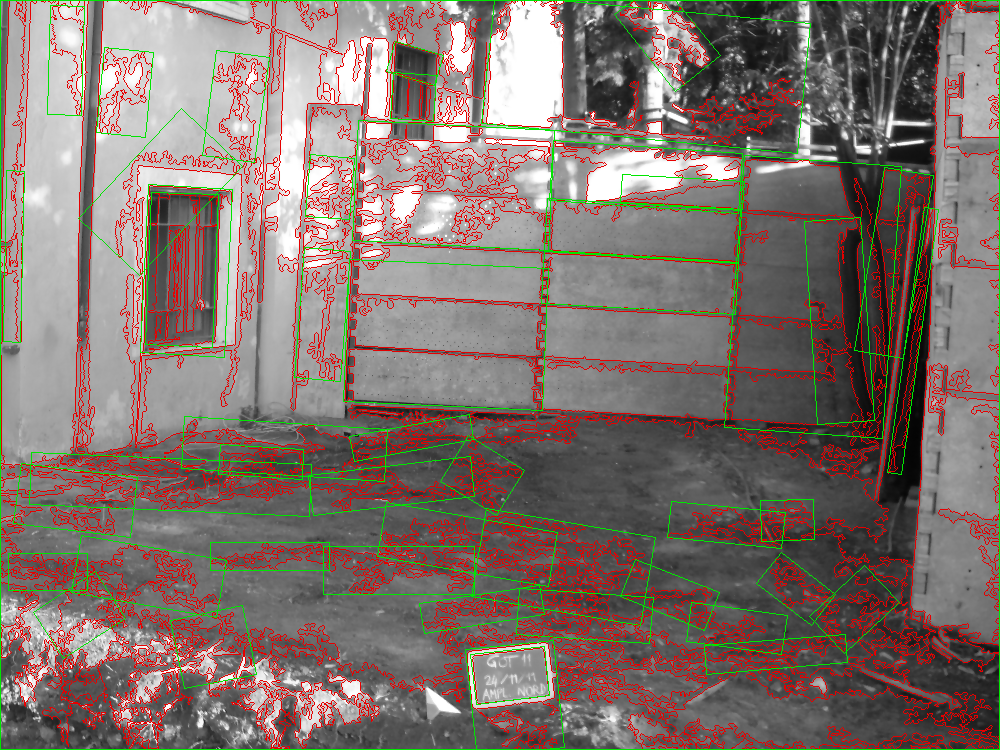
\includegraphics[width =0.5\textwidth]{catacom_1111_adaptive_allrects.png}
\caption{Konturen ohne und mit Rechtecken.}
\label{fig:adaptiverectangles}
\end{figure}

Anschließend werden die bereits berechneten Flächen der Konturen mit denen der kleinstmöglichen Rechtecke verglichen. Die Annahme: Nähert sich der Flächeninhalt der Kontur dem des Rechtecks an, handelt es sich bei der Kontur selbst wahrscheinlich um ein Rechteck. Als Grenzwert hat sich ein Verhältnis von 0.85 bewährt. Ebenfalls ausgeschlossen wird ein Rechteck, wenn es die Fläche des gesamten Bildes ausmacht, da teilweise, wie auch bei diesem Beispiel, der Rand des Bildes als Kontur erkannt werden kann (Vgl. Abb. \ref{fig:adaptivrect}).
\begin{figure}[h!]
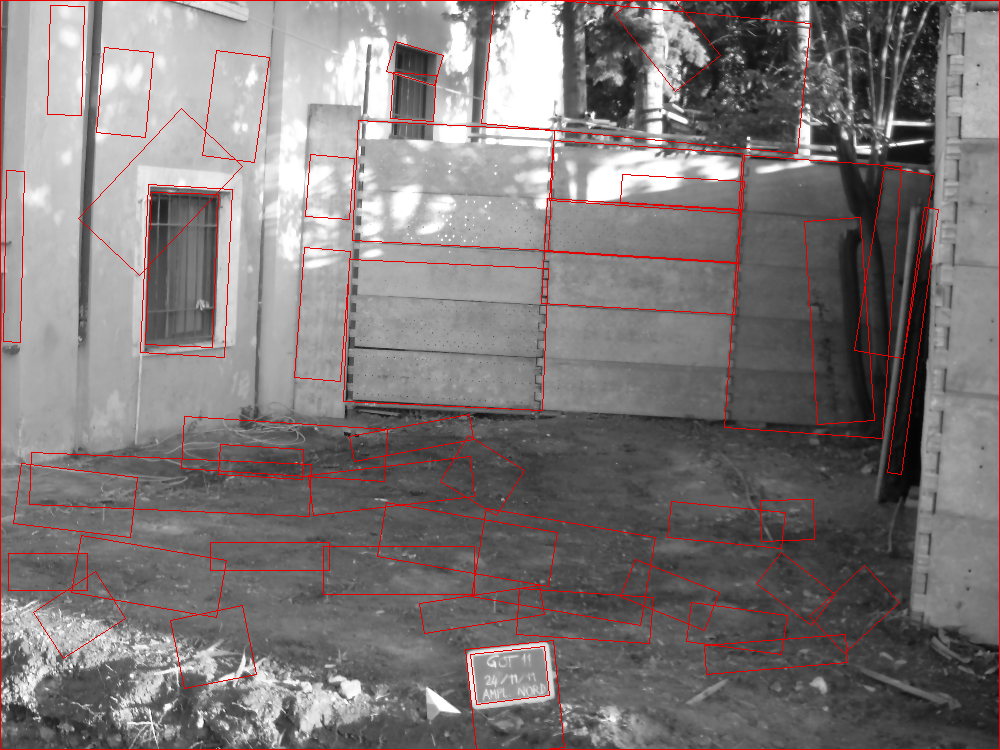
\includegraphics[width =0.5\textwidth]{catacom_1111_adaptive_allrectsred.png}
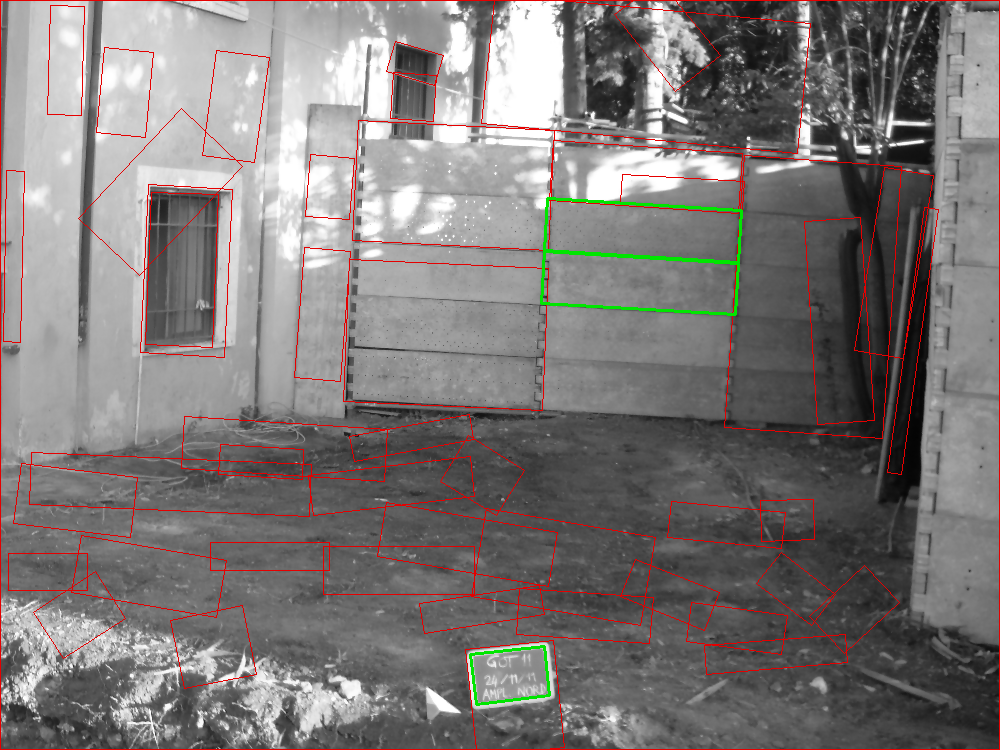
\includegraphics[width =0.5\textwidth]{catacom_1111_adaptive_rectarea.png}
\caption{Rechtecke aller Konturen und jene derer mit annähernd rechteckiger Fläche.}
\label{fig:adaptivrect}
\end{figure}

Als letztes Kriterium wird das Seitenverhältnis herangezogen. Im Programm besteht die Möglichkeit, vor der Untersuchung aller Bilder ein Template zu hinterlegen, auf dem eine Tafel gut und eindeutig zu sehen ist. Aus diesem Template wird das Seitenverhältnis der Tafel berechnet. Findet dieser Schritt nicht statt, wird ein maximales Seitenverhältnis von 2:1 angenommen, da Tafeln selten in länglichen Formaten zu finden sind\footnote{Sollte das Format einer Tafel doch einmal von dieser Annahme abweichen, lassen sich hier problemlos Anpassungen vornehmen.}. Mit einer deutlichen, aber bewährten Toleranz von 30\% in jede Richtung wird das Seitenverhältnis der verbliebenen Rechtecke mit dem des Templates verglichen. Sind die Werte sich ähnlich genug, wird das Rechteck als Tafel interpretiert und gilt als das Ergebnis des Algorithmus(Vgl. Abb. \ref{fig:aspectratio}).
\begin{figure}[h!]
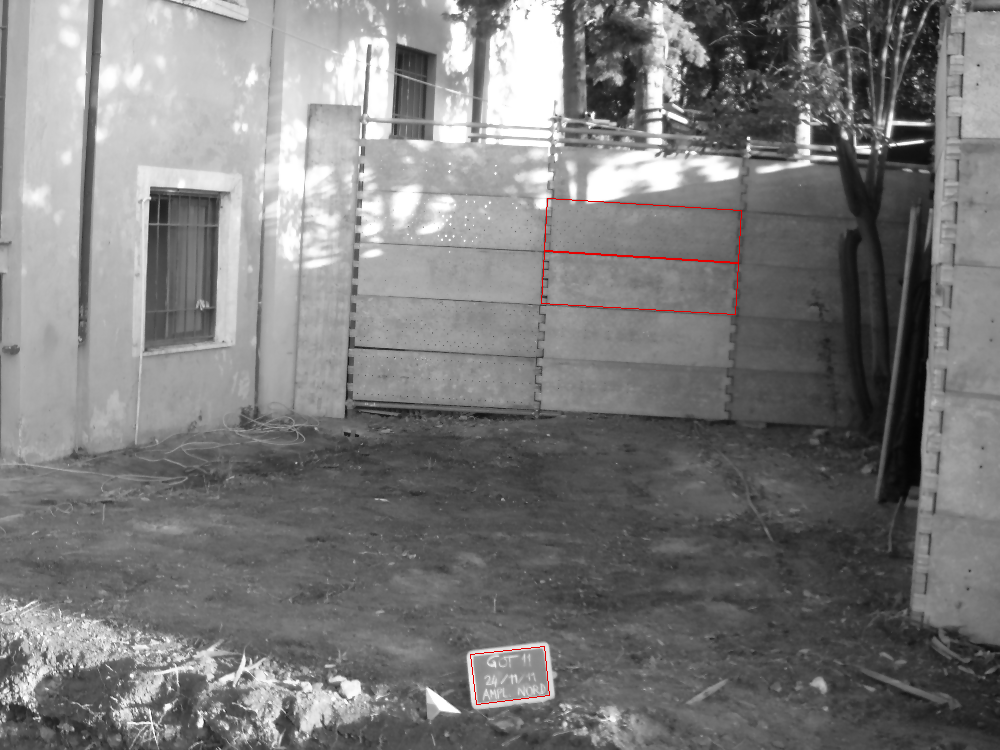
\includegraphics[width =0.5\textwidth]{catacom_1111_adaptive_rectareared.png}
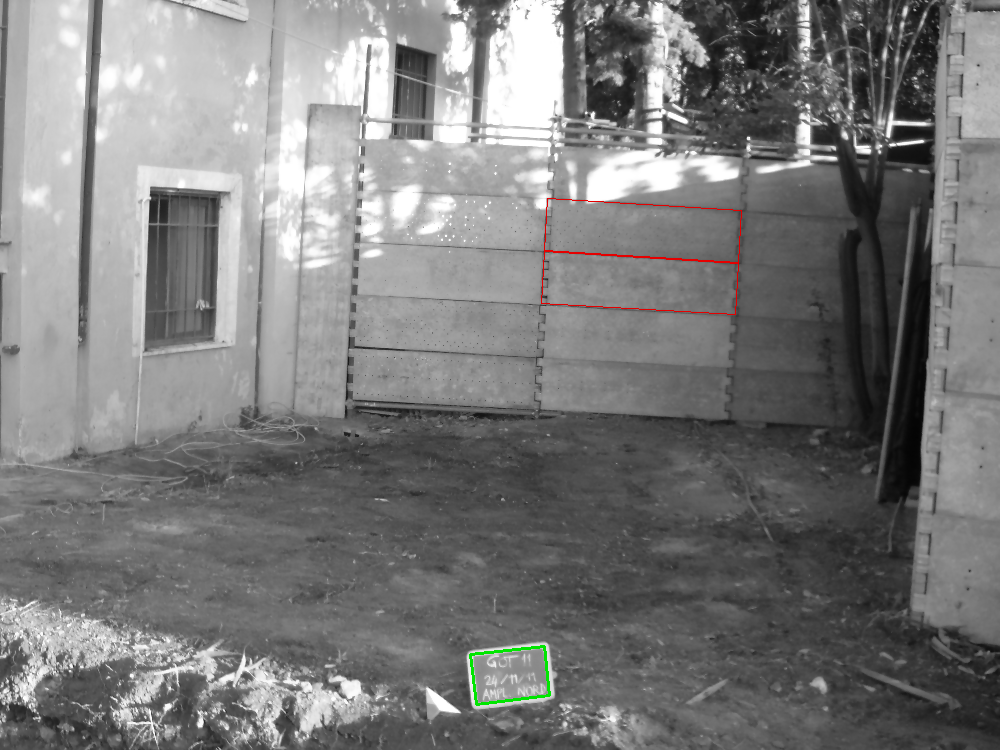
\includegraphics[width =0.5\textwidth]{catacom_1111_adaptive_aspectratio.png}
\caption{Die bisher verbliebenen Rechtecke und die mit dem richtigen Seitenverhältnis.}
\label{fig:aspectratio}
\end{figure}
 
\subsection{Cropverfahren}

Durch die vorhergehende Rechtecksdetektion sind die Positionen der Tafeln bekannt. Der nächste Schritt besteht darin, die Tafeln aus dem Gesamtbild auszuschneiden, damit diese Ausschnitte für die Texterkennung genutzt werden können. Dabei liegt Herausforderung nicht im Ausschneiden per se. Aufwändiger ist, das hier auch die perspektivischen Verzerrungen der Tafeln ausgeglichen werden müssen. Für diesen Ausgleich müssen die Eckpunkte der Tafeln bestimmt und das durch sie definierte Viereck auf die Fläche eines Rechtecks übertragen werden.
Auch hier haben sich wieder zwei Verfahren ergeben, von denen eines eher schnell und effizient arbeitet, während das zweite stärker auf das Entzerren der Bilder abzielt (Vgl. Abb. \ref{fig:flowchartcrop}). Beide Verfahren sollen im Folgenden vorgestellt und mit ihren Stärken und Schwächen diskutiert werden.
\begin{figure}[h!]
\centering
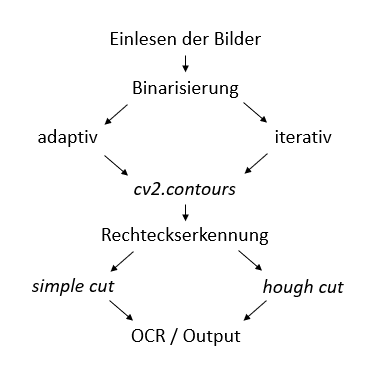
\includegraphics[width =0.5\textwidth]{flowchart_cont_crop.PNG}
\caption{Flowchart Crop-Verfahren.}
\label{fig:flowchartcrop}
\end{figure}
%Was ist die Aufgabe beim Crop?
%Worin liegen hier die Schwierigkeiten?
%Auch hier wieder Zweispurigkeit der Ansätze erklären

\subsubsection{simple crop}


Was ist die Idee?
Wie wurde sie umgesetzt?
Wo liegen die Probleme?

\subsubsection{Hough}

Was ist die Idee?
Wie wurde sie umgesetzt?
Wo liegen die Probleme?

\subsection{Experimentelles}

\subsection{Zusammenfassung}
evtl zusammenfassen wie vorgegangen wurde, warum dieser Weg gut ist und was das Wichtigste Ergebnis ist